% Created by tikzDevice version 0.10.1 on 2016-08-26 09:53:37
% !TEX encoding = UTF-8 Unicode
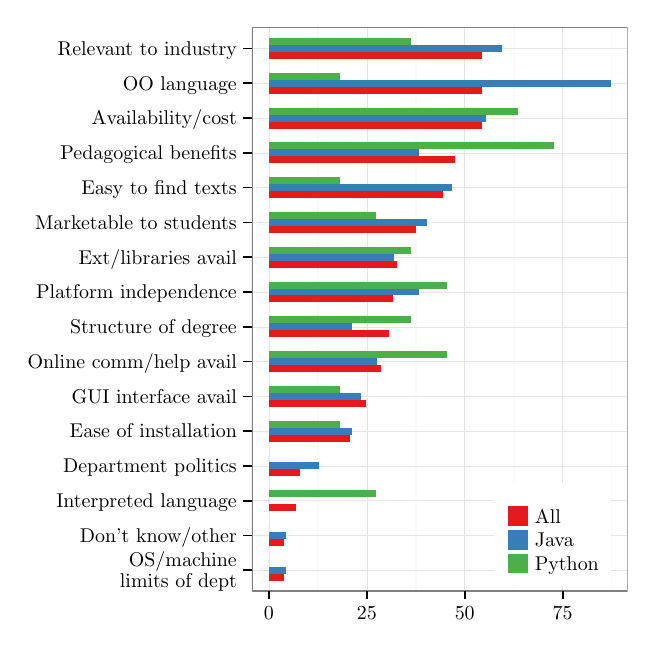
\begin{tikzpicture}[x=1pt,y=1pt]
\definecolor{fillColor}{RGB}{255,255,255}
\path[use as bounding box,fill=fillColor,fill opacity=0.00] (0,0) rectangle (216.81,216.81);
\begin{scope}
\path[clip] (  0.00,  0.00) rectangle (216.81,216.81);
\definecolor{drawColor}{RGB}{255,255,255}
\definecolor{fillColor}{RGB}{255,255,255}

\path[draw=drawColor,line width= 0.6pt,line join=round,line cap=round,fill=fillColor] (  0.00,  0.00) rectangle (216.81,216.81);
\end{scope}
\begin{scope}
\path[clip] ( 80.98, 13.20) rectangle (216.81,216.81);
\definecolor{fillColor}{RGB}{255,255,255}

\path[fill=fillColor] ( 80.98, 13.20) rectangle (216.81,216.81);
\definecolor{drawColor}{gray}{0.98}

\path[draw=drawColor,line width= 0.6pt,line join=round] (104.85, 13.20) --
	(104.85,216.81);

\path[draw=drawColor,line width= 0.6pt,line join=round] (140.24, 13.20) --
	(140.24,216.81);

\path[draw=drawColor,line width= 0.6pt,line join=round] (175.63, 13.20) --
	(175.63,216.81);

\path[draw=drawColor,line width= 0.6pt,line join=round] (211.02, 13.20) --
	(211.02,216.81);
\definecolor{drawColor}{gray}{0.90}

\path[draw=drawColor,line width= 0.2pt,line join=round] ( 80.98, 20.75) --
	(216.81, 20.75);

\path[draw=drawColor,line width= 0.2pt,line join=round] ( 80.98, 33.31) --
	(216.81, 33.31);

\path[draw=drawColor,line width= 0.2pt,line join=round] ( 80.98, 45.88) --
	(216.81, 45.88);

\path[draw=drawColor,line width= 0.2pt,line join=round] ( 80.98, 58.45) --
	(216.81, 58.45);

\path[draw=drawColor,line width= 0.2pt,line join=round] ( 80.98, 71.02) --
	(216.81, 71.02);

\path[draw=drawColor,line width= 0.2pt,line join=round] ( 80.98, 83.59) --
	(216.81, 83.59);

\path[draw=drawColor,line width= 0.2pt,line join=round] ( 80.98, 96.15) --
	(216.81, 96.15);

\path[draw=drawColor,line width= 0.2pt,line join=round] ( 80.98,108.72) --
	(216.81,108.72);

\path[draw=drawColor,line width= 0.2pt,line join=round] ( 80.98,121.29) --
	(216.81,121.29);

\path[draw=drawColor,line width= 0.2pt,line join=round] ( 80.98,133.86) --
	(216.81,133.86);

\path[draw=drawColor,line width= 0.2pt,line join=round] ( 80.98,146.43) --
	(216.81,146.43);

\path[draw=drawColor,line width= 0.2pt,line join=round] ( 80.98,159.00) --
	(216.81,159.00);

\path[draw=drawColor,line width= 0.2pt,line join=round] ( 80.98,171.56) --
	(216.81,171.56);

\path[draw=drawColor,line width= 0.2pt,line join=round] ( 80.98,184.13) --
	(216.81,184.13);

\path[draw=drawColor,line width= 0.2pt,line join=round] ( 80.98,196.70) --
	(216.81,196.70);

\path[draw=drawColor,line width= 0.2pt,line join=round] ( 80.98,209.27) --
	(216.81,209.27);

\path[draw=drawColor,line width= 0.2pt,line join=round] ( 87.16, 13.20) --
	( 87.16,216.81);

\path[draw=drawColor,line width= 0.2pt,line join=round] (122.54, 13.20) --
	(122.54,216.81);

\path[draw=drawColor,line width= 0.2pt,line join=round] (157.93, 13.20) --
	(157.93,216.81);

\path[draw=drawColor,line width= 0.2pt,line join=round] (193.32, 13.20) --
	(193.32,216.81);
\definecolor{fillColor}{RGB}{228,26,28}

\path[fill=fillColor] ( 87.16, 16.97) rectangle ( 92.76, 19.49);
\definecolor{fillColor}{RGB}{55,126,184}

\path[fill=fillColor] ( 87.16, 19.49) rectangle ( 93.19, 22.00);
\definecolor{fillColor}{RGB}{77,175,74}

\path[fill=fillColor] ( 87.16, 22.00) rectangle ( 87.16, 24.52);
\definecolor{fillColor}{RGB}{228,26,28}

\path[fill=fillColor] ( 87.16, 29.54) rectangle ( 92.76, 32.06);
\definecolor{fillColor}{RGB}{55,126,184}

\path[fill=fillColor] ( 87.16, 32.06) rectangle ( 93.19, 34.57);
\definecolor{fillColor}{RGB}{77,175,74}

\path[fill=fillColor] ( 87.16, 34.57) rectangle ( 87.16, 37.08);
\definecolor{fillColor}{RGB}{228,26,28}

\path[fill=fillColor] ( 87.16, 42.11) rectangle ( 96.97, 44.62);
\definecolor{fillColor}{RGB}{55,126,184}

\path[fill=fillColor] ( 87.16, 44.62) rectangle ( 87.16, 47.14);
\definecolor{fillColor}{RGB}{77,175,74}

\path[fill=fillColor] ( 87.16, 47.14) rectangle (125.76, 49.65);
\definecolor{fillColor}{RGB}{228,26,28}

\path[fill=fillColor] ( 87.16, 54.68) rectangle ( 98.37, 57.19);
\definecolor{fillColor}{RGB}{55,126,184}

\path[fill=fillColor] ( 87.16, 57.19) rectangle (105.23, 59.71);
\definecolor{fillColor}{RGB}{77,175,74}

\path[fill=fillColor] ( 87.16, 59.71) rectangle ( 87.16, 62.22);
\definecolor{fillColor}{RGB}{228,26,28}

\path[fill=fillColor] ( 87.16, 67.25) rectangle (116.59, 69.76);
\definecolor{fillColor}{RGB}{55,126,184}

\path[fill=fillColor] ( 87.16, 69.76) rectangle (117.28, 72.27);
\definecolor{fillColor}{RGB}{77,175,74}

\path[fill=fillColor] ( 87.16, 72.27) rectangle (112.89, 74.79);
\definecolor{fillColor}{RGB}{228,26,28}

\path[fill=fillColor] ( 87.16, 79.82) rectangle (122.19, 82.33);
\definecolor{fillColor}{RGB}{55,126,184}

\path[fill=fillColor] ( 87.16, 82.33) rectangle (120.28, 84.84);
\definecolor{fillColor}{RGB}{77,175,74}

\path[fill=fillColor] ( 87.16, 84.84) rectangle (112.89, 87.36);
\definecolor{fillColor}{RGB}{228,26,28}

\path[fill=fillColor] ( 87.16, 92.38) rectangle (127.80, 94.90);
\definecolor{fillColor}{RGB}{55,126,184}

\path[fill=fillColor] ( 87.16, 94.90) rectangle (126.31, 97.41);
\definecolor{fillColor}{RGB}{77,175,74}

\path[fill=fillColor] ( 87.16, 97.41) rectangle (151.49, 99.93);
\definecolor{fillColor}{RGB}{228,26,28}

\path[fill=fillColor] ( 87.16,104.95) rectangle (130.60,107.47);
\definecolor{fillColor}{RGB}{55,126,184}

\path[fill=fillColor] ( 87.16,107.47) rectangle (117.28,109.98);
\definecolor{fillColor}{RGB}{77,175,74}

\path[fill=fillColor] ( 87.16,109.98) rectangle (138.63,112.49);
\definecolor{fillColor}{RGB}{228,26,28}

\path[fill=fillColor] ( 87.16,117.52) rectangle (132.00,120.03);
\definecolor{fillColor}{RGB}{55,126,184}

\path[fill=fillColor] ( 87.16,120.03) rectangle (141.37,122.55);
\definecolor{fillColor}{RGB}{77,175,74}

\path[fill=fillColor] ( 87.16,122.55) rectangle (151.49,125.06);
\definecolor{fillColor}{RGB}{228,26,28}

\path[fill=fillColor] ( 87.16,130.09) rectangle (133.40,132.60);
\definecolor{fillColor}{RGB}{55,126,184}

\path[fill=fillColor] ( 87.16,132.60) rectangle (132.33,135.12);
\definecolor{fillColor}{RGB}{77,175,74}

\path[fill=fillColor] ( 87.16,135.12) rectangle (138.63,137.63);
\definecolor{fillColor}{RGB}{228,26,28}

\path[fill=fillColor] ( 87.16,142.66) rectangle (140.41,145.17);
\definecolor{fillColor}{RGB}{55,126,184}

\path[fill=fillColor] ( 87.16,145.17) rectangle (144.39,147.68);
\definecolor{fillColor}{RGB}{77,175,74}

\path[fill=fillColor] ( 87.16,147.68) rectangle (125.76,150.20);
\definecolor{fillColor}{RGB}{228,26,28}

\path[fill=fillColor] ( 87.16,155.23) rectangle (150.22,157.74);
\definecolor{fillColor}{RGB}{55,126,184}

\path[fill=fillColor] ( 87.16,157.74) rectangle (153.42,160.25);
\definecolor{fillColor}{RGB}{77,175,74}

\path[fill=fillColor] ( 87.16,160.25) rectangle (112.89,162.77);
\definecolor{fillColor}{RGB}{228,26,28}

\path[fill=fillColor] ( 87.16,167.79) rectangle (154.42,170.31);
\definecolor{fillColor}{RGB}{55,126,184}

\path[fill=fillColor] ( 87.16,170.31) rectangle (141.37,172.82);
\definecolor{fillColor}{RGB}{77,175,74}

\path[fill=fillColor] ( 87.16,172.82) rectangle (190.11,175.33);
\definecolor{fillColor}{RGB}{228,26,28}

\path[fill=fillColor] ( 87.16,180.36) rectangle (164.25,182.88);
\definecolor{fillColor}{RGB}{55,126,184}

\path[fill=fillColor] ( 87.16,182.88) rectangle (165.47,185.39);
\definecolor{fillColor}{RGB}{77,175,74}

\path[fill=fillColor] ( 87.16,185.39) rectangle (177.24,187.90);
\definecolor{fillColor}{RGB}{228,26,28}

\path[fill=fillColor] ( 87.16,192.93) rectangle (164.25,195.44);
\definecolor{fillColor}{RGB}{55,126,184}

\path[fill=fillColor] ( 87.16,195.44) rectangle (210.64,197.96);
\definecolor{fillColor}{RGB}{77,175,74}

\path[fill=fillColor] ( 87.16,197.96) rectangle (112.89,200.47);
\definecolor{fillColor}{RGB}{228,26,28}

\path[fill=fillColor] ( 87.16,205.50) rectangle (164.25,208.01);
\definecolor{fillColor}{RGB}{55,126,184}

\path[fill=fillColor] ( 87.16,208.01) rectangle (171.48,210.53);
\definecolor{fillColor}{RGB}{77,175,74}

\path[fill=fillColor] ( 87.16,210.53) rectangle (138.63,213.04);
\definecolor{drawColor}{gray}{0.50}

\path[draw=drawColor,line width= 0.6pt,line join=round,line cap=round] ( 80.98, 13.20) rectangle (216.81,216.81);
\end{scope}
\begin{scope}
\path[clip] (  0.00,  0.00) rectangle (216.81,216.81);
\definecolor{drawColor}{RGB}{0,0,0}

\node[text=drawColor,anchor=base east,inner sep=0pt, outer sep=0pt, scale=  0.72] at ( 75.58, 22.15) {OS/machine};

\node[text=drawColor,anchor=base east,inner sep=0pt, outer sep=0pt, scale=  0.72] at ( 75.58, 14.38) {limits of dept};

\node[text=drawColor,anchor=base east,inner sep=0pt, outer sep=0pt, scale=  0.72] at ( 75.58, 30.83) {Don't know/other};

\node[text=drawColor,anchor=base east,inner sep=0pt, outer sep=0pt, scale=  0.72] at ( 75.58, 43.40) {Interpreted language};

\node[text=drawColor,anchor=base east,inner sep=0pt, outer sep=0pt, scale=  0.72] at ( 75.58, 55.97) {Department politics};

\node[text=drawColor,anchor=base east,inner sep=0pt, outer sep=0pt, scale=  0.72] at ( 75.58, 68.54) {Ease of installation};

\node[text=drawColor,anchor=base east,inner sep=0pt, outer sep=0pt, scale=  0.72] at ( 75.58, 81.11) {GUI interface avail};

\node[text=drawColor,anchor=base east,inner sep=0pt, outer sep=0pt, scale=  0.72] at ( 75.58, 93.68) {Online comm/help avail};

\node[text=drawColor,anchor=base east,inner sep=0pt, outer sep=0pt, scale=  0.72] at ( 75.58,106.24) {Structure of degree};

\node[text=drawColor,anchor=base east,inner sep=0pt, outer sep=0pt, scale=  0.72] at ( 75.58,118.81) {Platform independence};

\node[text=drawColor,anchor=base east,inner sep=0pt, outer sep=0pt, scale=  0.72] at ( 75.58,131.38) {Ext/libraries avail};

\node[text=drawColor,anchor=base east,inner sep=0pt, outer sep=0pt, scale=  0.72] at ( 75.58,143.95) {Marketable to students};

\node[text=drawColor,anchor=base east,inner sep=0pt, outer sep=0pt, scale=  0.72] at ( 75.58,156.52) {Easy to find texts};

\node[text=drawColor,anchor=base east,inner sep=0pt, outer sep=0pt, scale=  0.72] at ( 75.58,169.08) {Pedagogical benefits};

\node[text=drawColor,anchor=base east,inner sep=0pt, outer sep=0pt, scale=  0.72] at ( 75.58,181.65) {Availability/cost};

\node[text=drawColor,anchor=base east,inner sep=0pt, outer sep=0pt, scale=  0.72] at ( 75.58,194.22) {OO language};

\node[text=drawColor,anchor=base east,inner sep=0pt, outer sep=0pt, scale=  0.72] at ( 75.58,206.79) {Relevant to industry};
\end{scope}
\begin{scope}
\path[clip] (  0.00,  0.00) rectangle (216.81,216.81);
\definecolor{drawColor}{RGB}{0,0,0}

\path[draw=drawColor,line width= 0.6pt,line join=round] ( 77.98, 20.75) --
	( 80.98, 20.75);

\path[draw=drawColor,line width= 0.6pt,line join=round] ( 77.98, 33.31) --
	( 80.98, 33.31);

\path[draw=drawColor,line width= 0.6pt,line join=round] ( 77.98, 45.88) --
	( 80.98, 45.88);

\path[draw=drawColor,line width= 0.6pt,line join=round] ( 77.98, 58.45) --
	( 80.98, 58.45);

\path[draw=drawColor,line width= 0.6pt,line join=round] ( 77.98, 71.02) --
	( 80.98, 71.02);

\path[draw=drawColor,line width= 0.6pt,line join=round] ( 77.98, 83.59) --
	( 80.98, 83.59);

\path[draw=drawColor,line width= 0.6pt,line join=round] ( 77.98, 96.15) --
	( 80.98, 96.15);

\path[draw=drawColor,line width= 0.6pt,line join=round] ( 77.98,108.72) --
	( 80.98,108.72);

\path[draw=drawColor,line width= 0.6pt,line join=round] ( 77.98,121.29) --
	( 80.98,121.29);

\path[draw=drawColor,line width= 0.6pt,line join=round] ( 77.98,133.86) --
	( 80.98,133.86);

\path[draw=drawColor,line width= 0.6pt,line join=round] ( 77.98,146.43) --
	( 80.98,146.43);

\path[draw=drawColor,line width= 0.6pt,line join=round] ( 77.98,159.00) --
	( 80.98,159.00);

\path[draw=drawColor,line width= 0.6pt,line join=round] ( 77.98,171.56) --
	( 80.98,171.56);

\path[draw=drawColor,line width= 0.6pt,line join=round] ( 77.98,184.13) --
	( 80.98,184.13);

\path[draw=drawColor,line width= 0.6pt,line join=round] ( 77.98,196.70) --
	( 80.98,196.70);

\path[draw=drawColor,line width= 0.6pt,line join=round] ( 77.98,209.27) --
	( 80.98,209.27);
\end{scope}
\begin{scope}
\path[clip] (  0.00,  0.00) rectangle (216.81,216.81);
\definecolor{drawColor}{RGB}{0,0,0}

\path[draw=drawColor,line width= 0.6pt,line join=round] ( 87.16, 10.20) --
	( 87.16, 13.20);

\path[draw=drawColor,line width= 0.6pt,line join=round] (122.54, 10.20) --
	(122.54, 13.20);

\path[draw=drawColor,line width= 0.6pt,line join=round] (157.93, 10.20) --
	(157.93, 13.20);

\path[draw=drawColor,line width= 0.6pt,line join=round] (193.32, 10.20) --
	(193.32, 13.20);
\end{scope}
\begin{scope}
\path[clip] (  0.00,  0.00) rectangle (216.81,216.81);
\definecolor{drawColor}{RGB}{0,0,0}

\node[text=drawColor,anchor=base,inner sep=0pt, outer sep=0pt, scale=  0.72] at ( 87.16,  2.85) {0};

\node[text=drawColor,anchor=base,inner sep=0pt, outer sep=0pt, scale=  0.72] at (122.54,  2.85) {25};

\node[text=drawColor,anchor=base,inner sep=0pt, outer sep=0pt, scale=  0.72] at (157.93,  2.85) {50};

\node[text=drawColor,anchor=base,inner sep=0pt, outer sep=0pt, scale=  0.72] at (193.32,  2.85) {75};
\end{scope}
\begin{scope}
\path[clip] (  0.00,  0.00) rectangle (216.81,216.81);
\definecolor{fillColor}{RGB}{255,255,255}

\path[fill=fillColor] (168.66, 14.69) rectangle (210.63, 52.44);
\end{scope}
\begin{scope}
\path[clip] (  0.00,  0.00) rectangle (216.81,216.81);
\definecolor{fillColor}{RGB}{228,26,28}

\path[fill=fillColor] (173.64, 36.74) rectangle (180.75, 43.85);
\end{scope}
\begin{scope}
\path[clip] (  0.00,  0.00) rectangle (216.81,216.81);
\definecolor{fillColor}{RGB}{55,126,184}

\path[fill=fillColor] (173.64, 28.20) rectangle (180.75, 35.31);
\end{scope}
\begin{scope}
\path[clip] (  0.00,  0.00) rectangle (216.81,216.81);
\definecolor{fillColor}{RGB}{77,175,74}

\path[fill=fillColor] (173.64, 19.67) rectangle (180.75, 26.78);
\end{scope}
\begin{scope}
\path[clip] (  0.00,  0.00) rectangle (216.81,216.81);
\definecolor{drawColor}{RGB}{0,0,0}

\node[text=drawColor,anchor=base west,inner sep=0pt, outer sep=0pt, scale=  0.72] at (183.27, 37.81) {All};
\end{scope}
\begin{scope}
\path[clip] (  0.00,  0.00) rectangle (216.81,216.81);
\definecolor{drawColor}{RGB}{0,0,0}

\node[text=drawColor,anchor=base west,inner sep=0pt, outer sep=0pt, scale=  0.72] at (183.27, 29.28) {Java};
\end{scope}
\begin{scope}
\path[clip] (  0.00,  0.00) rectangle (216.81,216.81);
\definecolor{drawColor}{RGB}{0,0,0}

\node[text=drawColor,anchor=base west,inner sep=0pt, outer sep=0pt, scale=  0.72] at (183.27, 20.74) {Python};
\end{scope}
\end{tikzpicture}
